\chapter{Basisarchitektur für ein sicheres Netzwerk}
Die Grundarchitektur für ein sicheres Netzwerk umfasst laut Bundesamt für Sicherheit in der Informationstechnik (BSI) 3 Zonen \cite{isi-lana}: 
\begin{itemize}
	\item das Interne Netz 
	\item das Sicherheitsgateway
	\item sowie die Internet Anbindung	
\end{itemize}
Abbildung \ref{grundarch} zeigt diesen Aufbau. Das \emph{Local Area Network} (\emph{LAN}) besteht aus mehreren, physikalisch durch einen Paketfilter getrennten, Subnetzen. Hier sollten sich zumindest die Server und die Clientrechner in eigenen Subnetzen befinden, sowie Rechner mit unterschiedlich hohem Schutzbedarf. 

\begin{figure}
	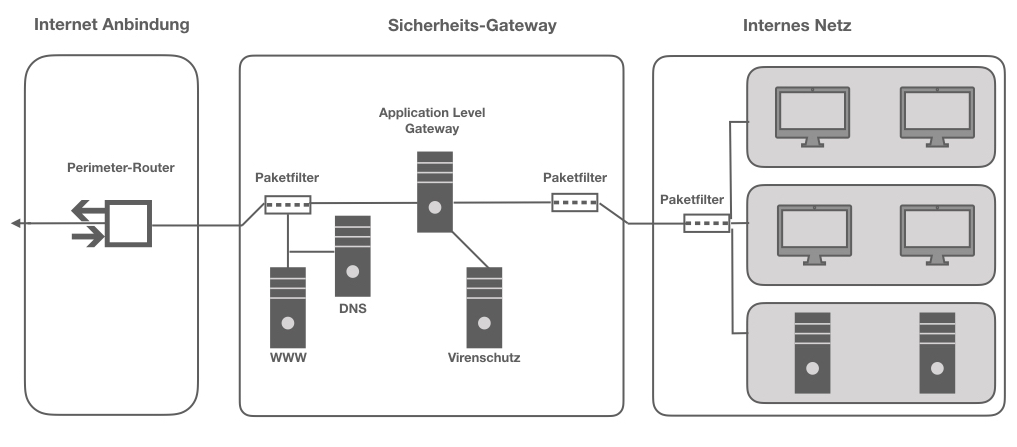
\includegraphics[width=\linewidth]{grundarchitektur}
	\caption{Grundarchitektur eines sicheren Netzwerkes}
	\label{grundarch}
\end{figure}

Die zwiete Zone, das Sicherheitsgateway, trennt die InternetAnbindung vom internen Firmennetz. Hier wird eine P-A-P Struktur empfohlen, bestehend aus einem Paketfilter auf der Seite des lokalen Netzes, sowie einem Paketfilter auf Seite des Internets, die jeweils die Kommunikation auf der dritten Schicht des Protokollstapel, der Vermittlungsschicht oder auch IP-Schicht, filtern. Der Paketfilter auf Seiten des LANs untersucht die nach außen gerichteten Pakete, der Paketfilter auf Seiten der Internetanbindung filtert die ankommenden IP-Pakete.

\begin{figure}
	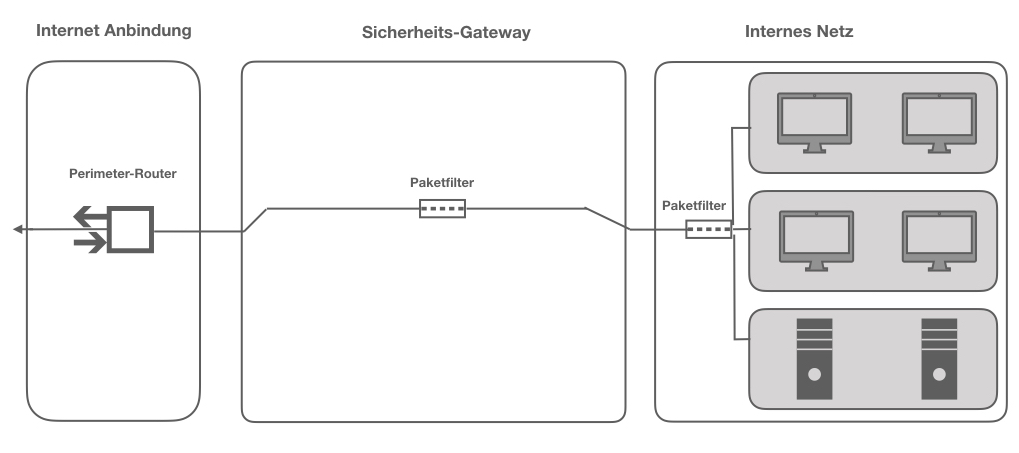
\includegraphics[width=\linewidth]{klUnternHoch.jpeg}
	\caption{Grundarchitektur für ein kleines Unternehmen mit normalem Schutzbedarf}
	\label{klUnorm}
\end{figure}

\begin{figure}
	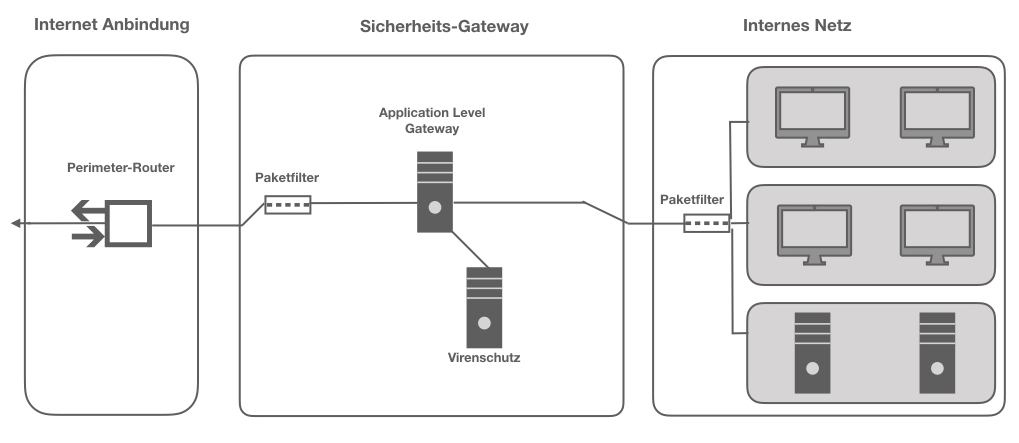
\includegraphics[width= \linewidth]{klUnternehmnorm}
	\caption{Grundarchitektur für ein kleines Unternehmen mit hohem Schutzbedarf}
	\label{klUhoch}
\end{figure}